%% 
%% Copyright 2007, 2008, 2009 Elsevier Ltd
%% 
%% This file is part of the 'Elsarticle Bundle'.
%% ---------------------------------------------
%% 
%% It may be distributed under the conditions of the LaTeX Project Public
%% License, either version 1.2 of this license or (at your option) any
%% later version.  The latest version of this license is in
%%    http://www.latex-project.org/lppl.txt
%% and version 1.2 or later is part of all distributions of LaTeX
%% version 1999/12/01 or later.
%% 
%% The list of all files belonging to the 'Elsarticle Bundle' is
%% given in the file `manifest.txt'.
%% 

%% Template article for Elsevier's document class `elsarticle'
%% with numbered style bibliographic references
%% SP 2008/03/01

\documentclass[preprint,1p]{elsarticle}
\biboptions{numbers,sort&compress}

%% Use the option review to obtain double line spacing
%% \documentclass[authoryear,preprint,review,12pt]{elsarticle}

%% Use the options 1p,twocolumn; 3p; 3p,twocolumn; 5p; or 5p,twocolumn
%% for a journal layout:
%% \documentclass[final,1p,times]{elsarticle}
%% \documentclass[final,1p,times,twocolumn]{elsarticle}
%% \documentclass[final,3p,times]{elsarticle}
%% \documentclass[final,3p,times,twocolumn]{elsarticle}
%% \documentclass[final,5p,times]{elsarticle}
%% \documentclass[final,5p,times,twocolumn]{elsarticle}

%% For including figures, graphicx.sty has been loaded in
%% elsarticle.cls. If you prefer to use the old commands
%% please give \usepackage{epsfig}

%% The amssymb package provides various useful mathematical symbols
\usepackage{amssymb}
\usepackage{lineno}
\usepackage{hyperref}
\usepackage[percent]{overpic}
\usepackage[usenames,dvipsnames,svgnames,table]{xcolor}

%% The amsthm package provides extended theorem environments
%% \usepackage{amsthm}

%% The lineno packages adds line numbers. Start line numbering with
%% \begin{linenumbers}, end it with \end{linenumbers}. Or switch it on
%% for the whole article with \linenumbers.
%% \usepackage{lineno}

\journal{Nucl. Instrum. Meth. A}

\begin{document}
\linenumbers

\begin{frontmatter}

%% Title, authors and addresses

%% use the tnoteref command within \title for footnotes;
%% use the tnotetext command for theassociated footnote;
%% use the fnref command within \author or \address for footnotes;
%% use the fntext command for theassociated footnote;
%% use the corref command within \author for corresponding author footnotes;
%% use the cortext command for theassociated footnote;
%% use the ead command for the email address,
%% and the form \ead[url] for the home page:
%% \title{Title\tnoteref{label1}}
%% \tnotetext[label1]{}
%% \author{Name\corref{cor1}\fnref{label2}}
%% \ead{email address}
%% \ead[url]{home page}
%% \fntext[label2]{}
%% \cortext[cor1]{}
%% \address{Address\fnref{label3}}
%% \fntext[label3]{}

\title{Studies of uniformity of 50~$\mu$m UFSD sensors at the Fermilab test beam.}

%% use optional labels to link authors explicitly to addresses:
%% \author[label1,label2]{}
%% \address[label1]{}
%% \address[label2]{}

\author[1]{A.~Apresyan\corref{cor}}\ead{apresyan@fnal.gov}
\author[2]{S.~Xie}
\author[2]{C.~Pena}
\author[5,7]{R.~Arcidiacono}
\author[5]{N.~Cartiglia}
\author[8]{M.~Carulla}
\author[1]{G.~Derylo}
\author[5]{M.~Ferrero}
\author[8]{D.~Flores}
\author[4]{P.~Freeman}
\author[4]{Z.~Galloway}
%\author[4]{Y.~Ghao}
\author[9]{A.~Ghassemi}
\author[3]{H.~Al Ghoul}
\author[1]{L.~Gray}
\author[8]{S.~Hidalgo}
%\author[4]{C.~Labitan}
\author[9]{S.~Kamada}
\author[1]{S.~Los}
%\author[4]{Z.~Luce}
\author[5]{M.~Mandurrino}
\author[8]{A.~Merlos}
%\author[2]{A.~Mangu}
%\author[4]{F.~Martinez-Mckinney}
\author[3]{N.~Minafra}
%\author[1]{A.~Prosser}
%\author[1]{R.~Rivera}
\author[8]{G.~Pellegrini}
\author[8]{D.~Quirion}
\author[3]{C.~Royon}
\author[4]{H.~Sadrozinski}
\author[4]{A.~Seiden}
\author[5]{V.~Sola}
\author[2]{M.~Spiropulu}
%\author[4]{E.~Spencer}
\author[5]{A.~Staiano}
\author[1]{L.~Uplegger}
\author[9]{K.~Yamamoto}
\author[9]{K.~Yamamura}
%\author[4]{M.~Wilder}

\address[1]{Fermi National Accelerator Laboratory, Batavia, IL, USA}
\address[2]{California Institute of Technology, Pasadena, CA, USA}
\address[3]{University of Kansas, KS, USA}
\address[4]{SCIPP, University of California Santa Cruz, CA, USA}
\address[5]{INFN, Torino, Italy}
\address[6]{Universit\`a di Torino, Torino, Italy}
\address[7]{Universit\`a del Piemonte Orientale, Italy}
\address[8]{Centro Nacional de Microelectr\`onica (IMB-CNM-CSIC), Barcelona, Spain}
\address[9]{Hamamatsu Photonics (HPK), Hamamatsu, Japan}
\cortext[cor]{Corresponding author}

\begin{abstract}
%% Text of abstract
In this paper we report measurements of uniformity of time resolution, signal
amplitude, and charged particle detection efficiency across the sensor surface
of Ultra-Fast Silicon Detectors (UFSD). Comparisons of performance of sensors
with different doping concentrations, and different active thicknesses are
presented, as well as their temperature dependance and radiation tolerance up to
$6\times 10^{14}$~n/cm$^2$. Results were obtained at the Fermilab test beam
facility using 120 GeV proton beams, and a high precision pixel tracking
detector. UFSD sensors based on the Low-Gain Avalanche Detector (LGAD) design
were manufactured by the the Centro Nacional de Microelectr\`onica (CNM) and
Hamamatsu Photonics (HPK) were tested in the experiments. The uniformity of the
sensor response in pulse height, efficiency and timing resolution were found to
be good pre-radiation, with time resolution around 30-40~ps depending on
operating conditions. A ``no-response'' area between pads which exhibit was
measured to be around 70~$\mu$m for CNM and 110$\mu$m for HPK sensors. After a
neutron fluence of $6\times 10^{14}$~n/cm$^2$ the CNM sensor exhibits a large
gain variation of a factor 2.5 when comparing metallized and non-metallized
sensor areas. Irradiated CNM sensor achieved time resolution of 30~ps for the
metallized part, and 40~ps for the non-metallized area, while the time
resolution of the HPK sensor was measured to be 30~ps.

\end{abstract}

\begin{keyword}
%% keywords here, in the form: keyword \sep keyword

%% PACS codes here, in the form: \PACS code \sep code
Silicon \sep Timing \sep LGAD
%% MSC codes here, in the form: \MSC code \sep code
%% or \MSC[2008] code \sep code (2000 is the default)

\end{keyword}

\end{frontmatter}

%% \linenumbers

%% main text
\section{Introduction} 

Future colliders, including the high luminosity upgrade of the Large Hadron
Collider (HL-LHC) at CERN, will operate with an order of magnitude higher
instantaneous luminosity compared to what has been achieved at the LHC so far.
With the increased instantaneous luminosity the rate of simultaneous
interactions per bunch crossing (pileup) is projected to reach an average of 140
to 200. The large amount of pileup increases the likelihood of confusion in the
reconstruction of particles from the hard scatter interaction with those
produced in different pileup interactions. The ability to discriminate between
jets produced in the events of interests, especially those associated with the
vector boson fusion processes, and jets produced by pileup interactions will be
degraded. The efficiency of identifying high $p_{\mathrm{T}}$ isolated electrons
and muons will be severely reduced due to the high density of pileup particles
in their vicinity. The missing transverse energy resolution will deteriorate, and several
other physics objects performance metrics will suffer.

One way to mitigate the pileup confusion effects, complementary to precision
tracking methods, is to perform a time of arrival measurement associated with
each particle. Such a measurement with a precision of about 20-30~ps, will
reduce the effective amount of pileup by a factor of 10, given that the spread
in collision time of the pileup interactions at HL-LHC is foreseen to be
approximately 200~ps. We have previosuly shown that a precision of better than
$20$~ps can be achieved for electromagnetic showers measured with silicon
sampling calorimeters~\cite{Apresyan201662,Apresyan2017_NSSMIC,AKCHURIN201731}
using traditional planar silicon detectors. In this paper we report results of
beam test measurements with thin UFSD sensors that have been shown to achieve
time resolution around 30~ps~\cite{Cartiglia201783}. UFSD are envisioned to be
used in the CMS and ATLAS experiment upgrades for HL-LHC in order to reduce the
pileup contamination in the region of pseudorapidity beyond $\eta>1.5$ for CMS,
and $\eta>3.0$ for ATLAS. In order to satisfy the needs of a high precision
timing across a large area of the detectors for HL-LHC, the sensors will need to
be provide high uniformity of signal response and timing resolution. In this
paper we perform detailed measurements of the performance of UFSD sensors from
CNM and HPK exposed to the 120~GeV proton beams at Fermilab. Utilizing the high
precision tracking detector we extract position dependence of the timing
resolution, signal pulse height, signal time stamp, and charged particle
detection efficiency, as well as we compare the 50 and 80~$\mu$m UFSD sensors,
and the performance of the HPK and CNM sensors irradiated to $6\times
10^{14}$~n/cm$^2$.

The paper is organized as follows: the experimental setup is described in
Sec.~\ref{sec:setup}, the tested UFSD sensors and their operating conditions are
listed in Sec.~\ref{sec:sensors}, readout boards used in the measurements are described in Sec.~\ref{sec:boards}, beam test results are presented in Sec.~\ref{sec:results}, followed by the conclusion in Sec.~\ref{sec:conclusion}.

\section{Test-beam Setup} 
\label{sec:setup}

%We performed the test-beam measurements at the Fermilab Test-beam
%Facility%

Test-beam measurements were performed at the Fermilab Test-beam Facility (FTBF)
which provided a $120$~GeV proton beam from the Fermilab Main Injector
accelerator. The Devices Under Test (DUTs) were mounted on a remotely operated
motorized stage, placed inside the pixel telescope detector~\cite{KWAN2016162}.
The latter provides better than 10~$\mu$m position resolution for charged
particles impinging on the DUT. Additionally, a Photek~240 micro-channel plate
(MCP-PMT) detector~\cite{Anderson:2015gha, MCPFastCaloNIMA,
Ronzhin2015288,Ronzhin201552} was placed furthest downstream, and provided a
very precise reference timestamp. Its precision has been previously
measured to be less than $10$~ps~\cite{Ronzhin2015288}. A schematic diagram and
photograph of the experimental area are shown in Fig.~\ref{fig:DragonBoxDiagram}
and Fig.~\ref{fig:DragonBox}, respectively. 

The DAQ system for the DUTs and the Photek MCP-PMT is based on a CAEN V1742
digitizer board~\cite{CAENDRS}, which provides digitized waveforms sampled at 5
GS/s, and with one ADC count corresponding to 0.25~mV. The CAEN digitizer was
voltage- and time-calibrated using the procedure described in
Ref.~\cite{Kim201467}. The electronic€ time resolution of the CAEN V1742
digitizer was measured to be less than 4~ps, and thus, its impact on the timing
measurements presented in these studies can be neglected. The DAQ for the pixel
telescope is based on the CAPTAN system developed at
Fermilab~\cite{KWAN2016162}. The track-reconstruction is performed using the
Monicelli software package developed specifically for the test-beam application. 

The beam is resonantly extracted in a slow spill for each Main Injector cycle
delivering a single 4.2 sec long spill per minute. The primary beam (bunched at
53 MHz) consists of high energy protons (120 GeV) at variable intensities
between 1 and 300 kHz. The trigger to both the CAEN V1742 and to the pixel
telescope was provided by a scintillator mounted on a photomultiplier tube,
placed upstream of the DUTs in the beam-line. Due to the limited buffer depth of
the CAEN V1742 board, special care had to be taken in the design of the DAQ
system to ensure that both the DUT and telescope DAQs collect exactly the same
amount of triggers. This was achieved by limiting the trigger rate by
introducing an adjustable dead-time using a custom-designed trigger board. This
trigger board is the combination of a custom FPGA board (the CAPTAN+x, equipped
with multiple FPGA Mezzanine Card connectors and gigabit ethernet connectivity)
mated to a front end board (the NIM+, with multiple inputs and outputs, each
supporting a variety of interface levels such as NIM, LVDS, and TTL). The
combined board is shown in Fig.~\ref{fig:NIM+Captan} and was used to interface to
photomultiplier signals through on-board programmable discriminators, and to form
trigger signals with software configurable time-based veto and pre-scaler event
filtering. We found that at a rate of about 1,500 triggers per spill the CAEN
V1742 and pixel telescope were maintained fully synchronized. Processed data
from the pixel telescope and the DUTs were merged offline by matching the
trigger counters recorded by the two systems.

\begin{figure}[htbp] 
\centering
\includegraphics[width=0.5\textwidth, angle=270]{figs/CAPTAN_NIM_Plus.JPG} 
\caption{The custom-made trigger board composed of NIM+ and CAPTAN+x boards.} 
\label{fig:NIM+Captan} 
\end{figure} 




\begin{figure}[htbp] 
\centering
\includegraphics[width=0.75\textwidth]{figs/BeamSetup.pdf} 
\caption{A schematic diagram of the test-beam setup is shown. The $t_0$ and $t_1$ are defined in Section 4.} 
\label{fig:DragonBoxDiagram} 
\end{figure} 

The devices under test (DUT) were placed inside the telescope box described in
Ref.\cite{KWAN2016162}, and mounted on aluminum mechanical support structure.
The telescope box can be moved remotely in both horizontal and vertical
directions, in order to align the DUTs with the beam. The aluminum support
structures for DUT provide both a mechanical stability for the DUTs, and are
equipped with Peltier cooling elements that were used in this study to operate
the DUTs at $-10^{\circ}$ and $-20^{\circ}$~C.

\begin{figure}[htbp] 
\centering
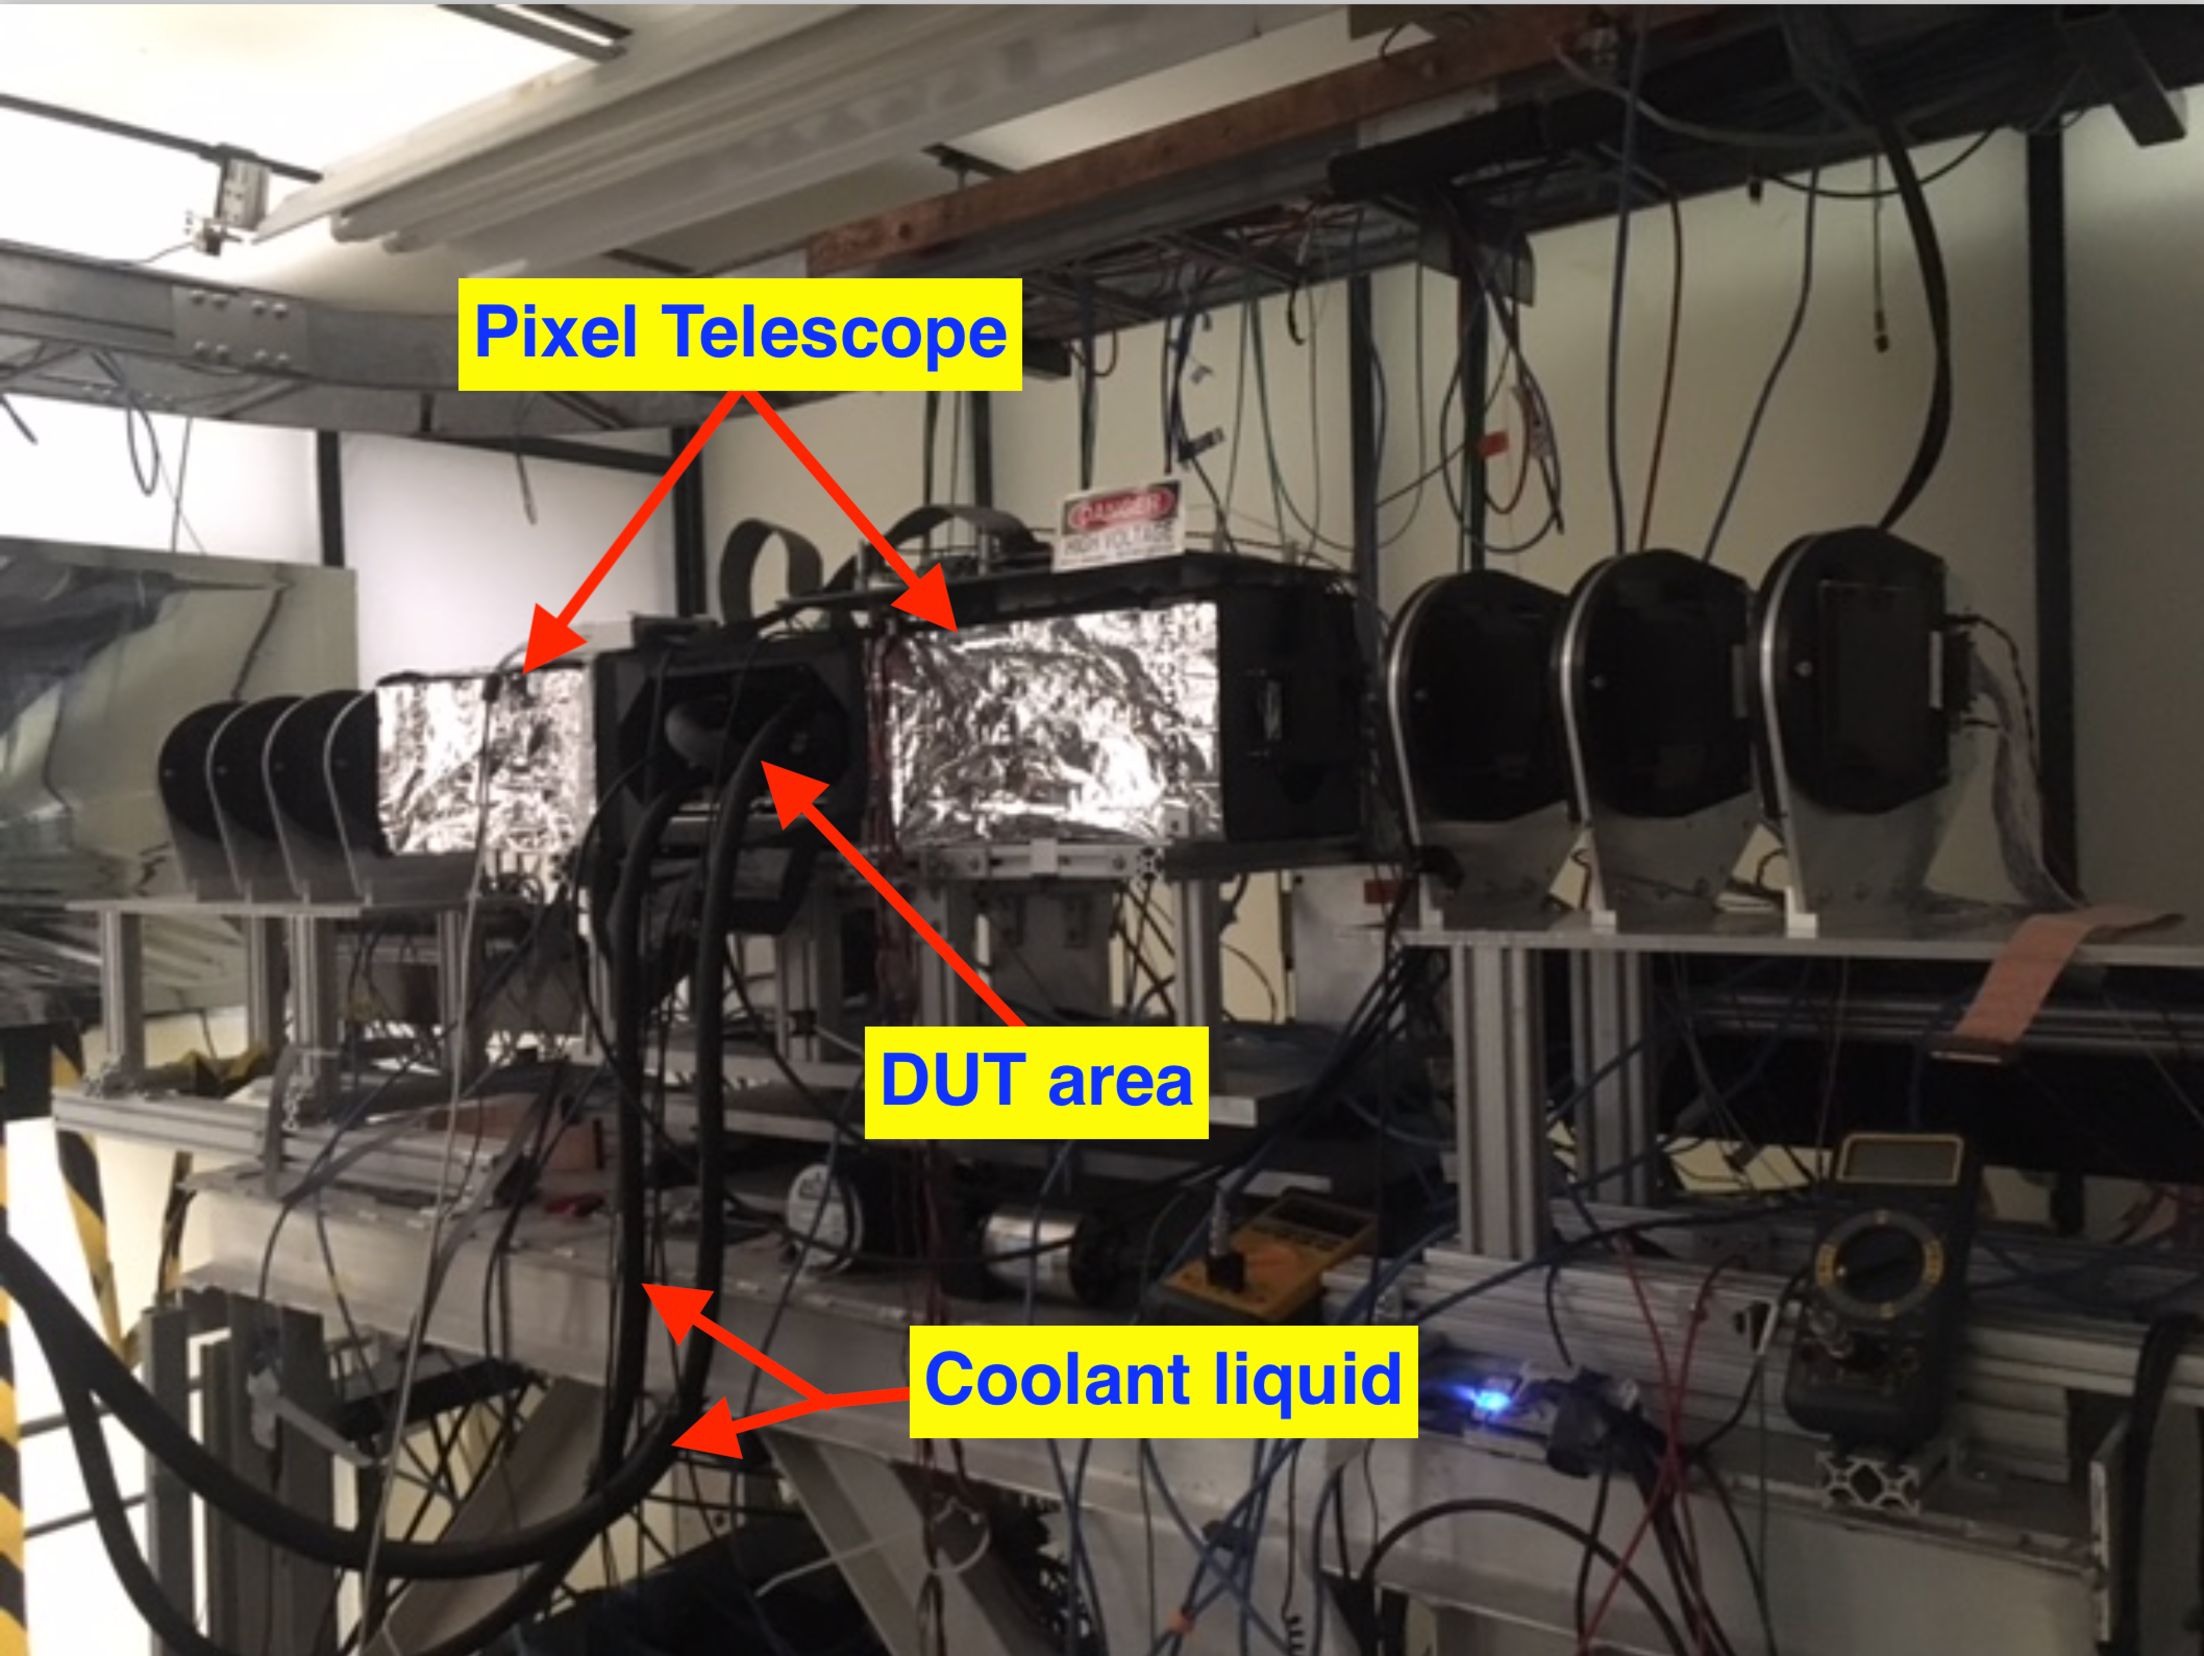
\includegraphics[width=0.75\textwidth]{figs/TB_dragonBox.pdf} 
\caption{A picture of the experimental area. Thea pixel telescope detectors are placed inside the ESD shielded boxes on the two sides of the DUT area. Cooling liquid for the Peltier elements inside the DUT area is provided by the two pipes shown in the picture.} 
\label{fig:DragonBox} 
\end{figure} 


\section{Properties of the tested LGAD sensors}
\label{sec:sensors}

Sensors manufactured by Hamamatsu (HPK) and CNM were tested during the test beam
experiments. Sensors in both single- and four-channel configurations were tested
during the measurements. Most of the tested sensors have active thickness of
about 50 $\mu$m, apart from the comparison of the 50 and 80 $\mu$m sensors that
is presented in Sec.~\ref{sec:HPK50vs80}. The list of sensors studied in this
article, as well as the temperature and the sensor bias voltage used during
their operation are listed in Tab.~\ref{tab:DataConditions}. 

CNM sensors have active thickness of about 45 $\mu$m, they were
produced on 4-inch Silicon-on-Insulator wafers with a 45 $\mu$m thick high
resistivity float zone (FZ) active layer on top of a 1 $\mu$m buried oxide and a
300 $\mu$m support wafer. The back-side contact is done through wet-etched deep
access holes through the insulator. Details on CNM sensors can be found in
Ref.~\cite{CNMSensors, Cartiglia201783}. 

The HPK sensors were manufactured on 6-inch silicon wafers of 150 $\mu$m total
thickness with a 50 $\mu$m or 80 $\mu$m thick high resistivity float zone (FZ)
active layer. Four gain splits, identified with the letters A (lowest gain) to D
(highest gain), were produced, identical in the mask design but with a different
$p^+$ dose of the gain layer, to study the optimum parameters of the charge
multiplication mechanism. The pads were produced in three versions: two with
guard ring (GR and GBGR) and one without guard ring. Four-channel sensors in 2x2
array were produced with all 4 gain-splits, and are identified with the PIX
identifier, e.g. the 2x2 array of the 50 $\mu$m sensor split D is labelled as
50D-PIX. 

Each channel in the 2x2 HPK array is 3x3~mm$^2$. The CNM single-channel sensors
are square pads with an active area of 1.7 mm$^2$ while the HPK single-channel
sensors are circular pads with an active area of 0.8~mm$^2$.

\begin{figure}[!htbp] 
\centering
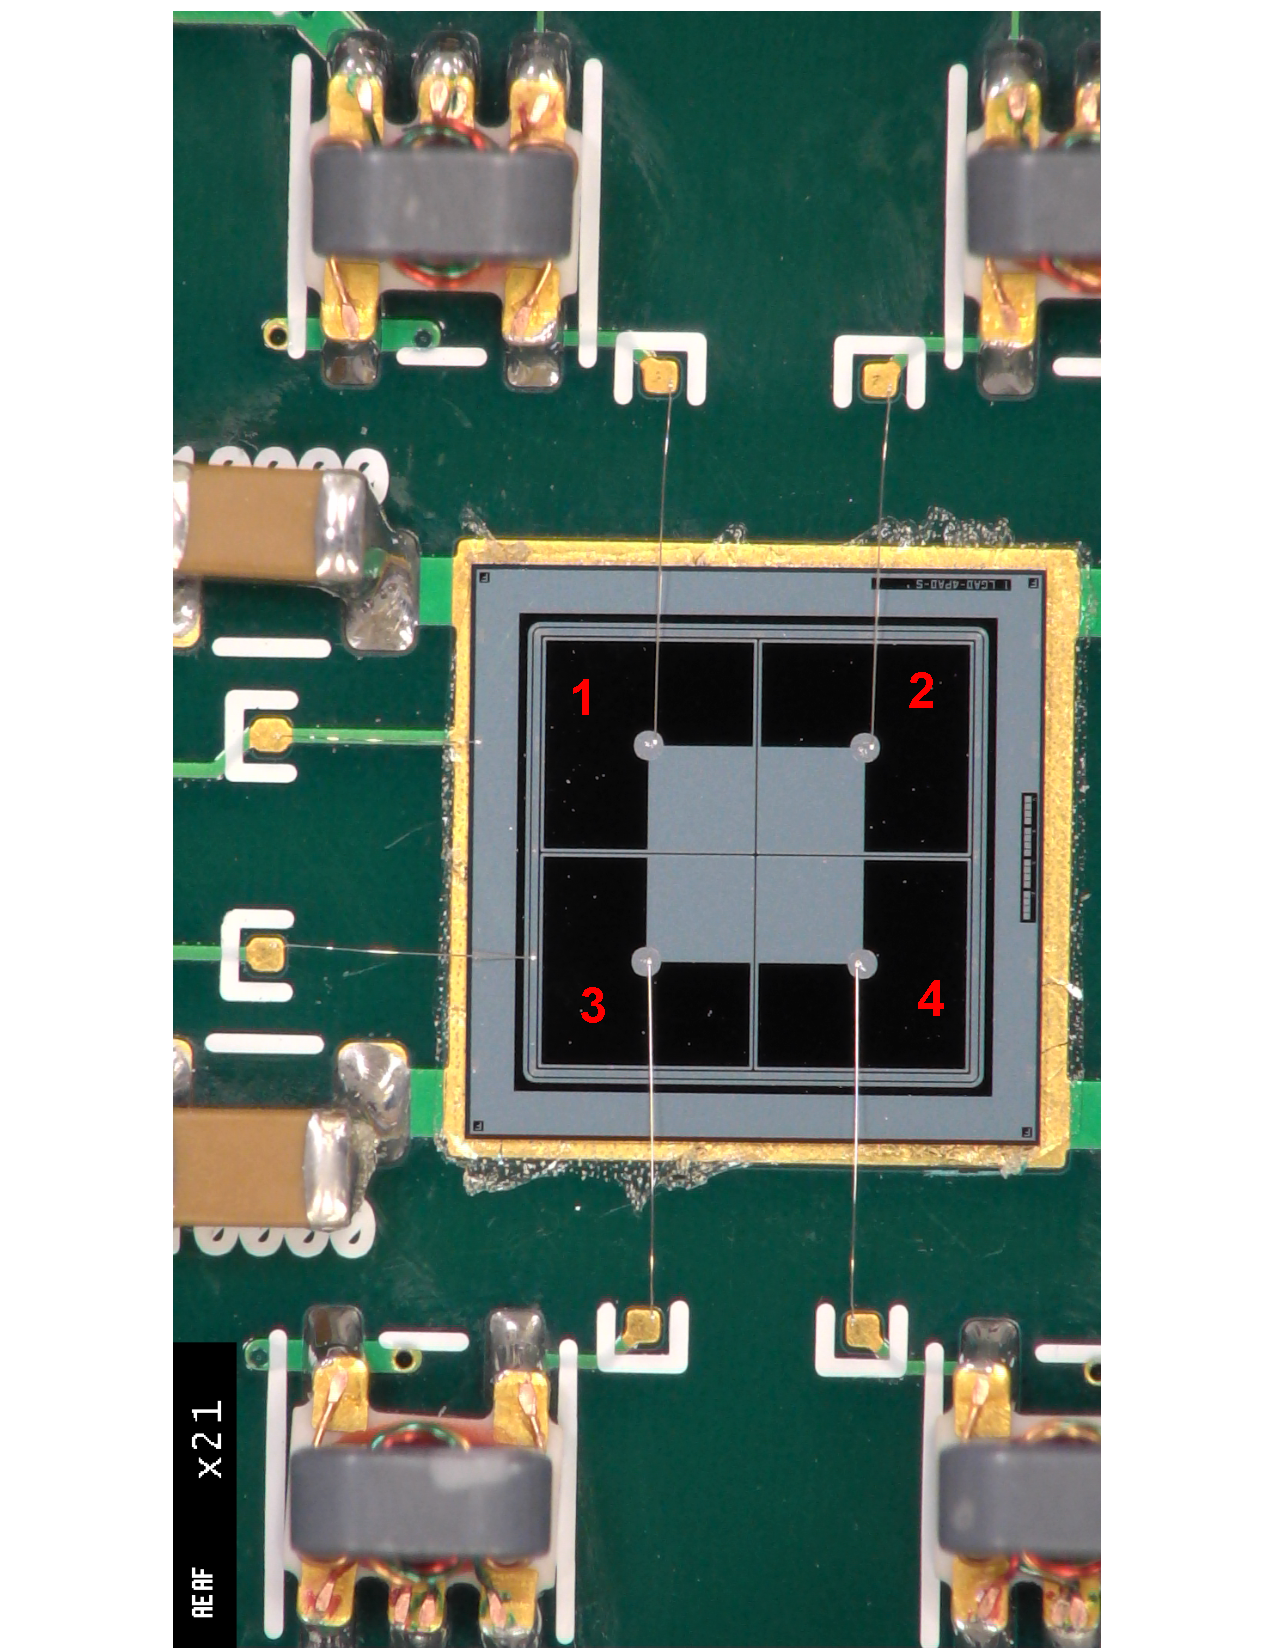
\includegraphics[width=0.3\textwidth]{figs/HPK-50DPix.pdf} 
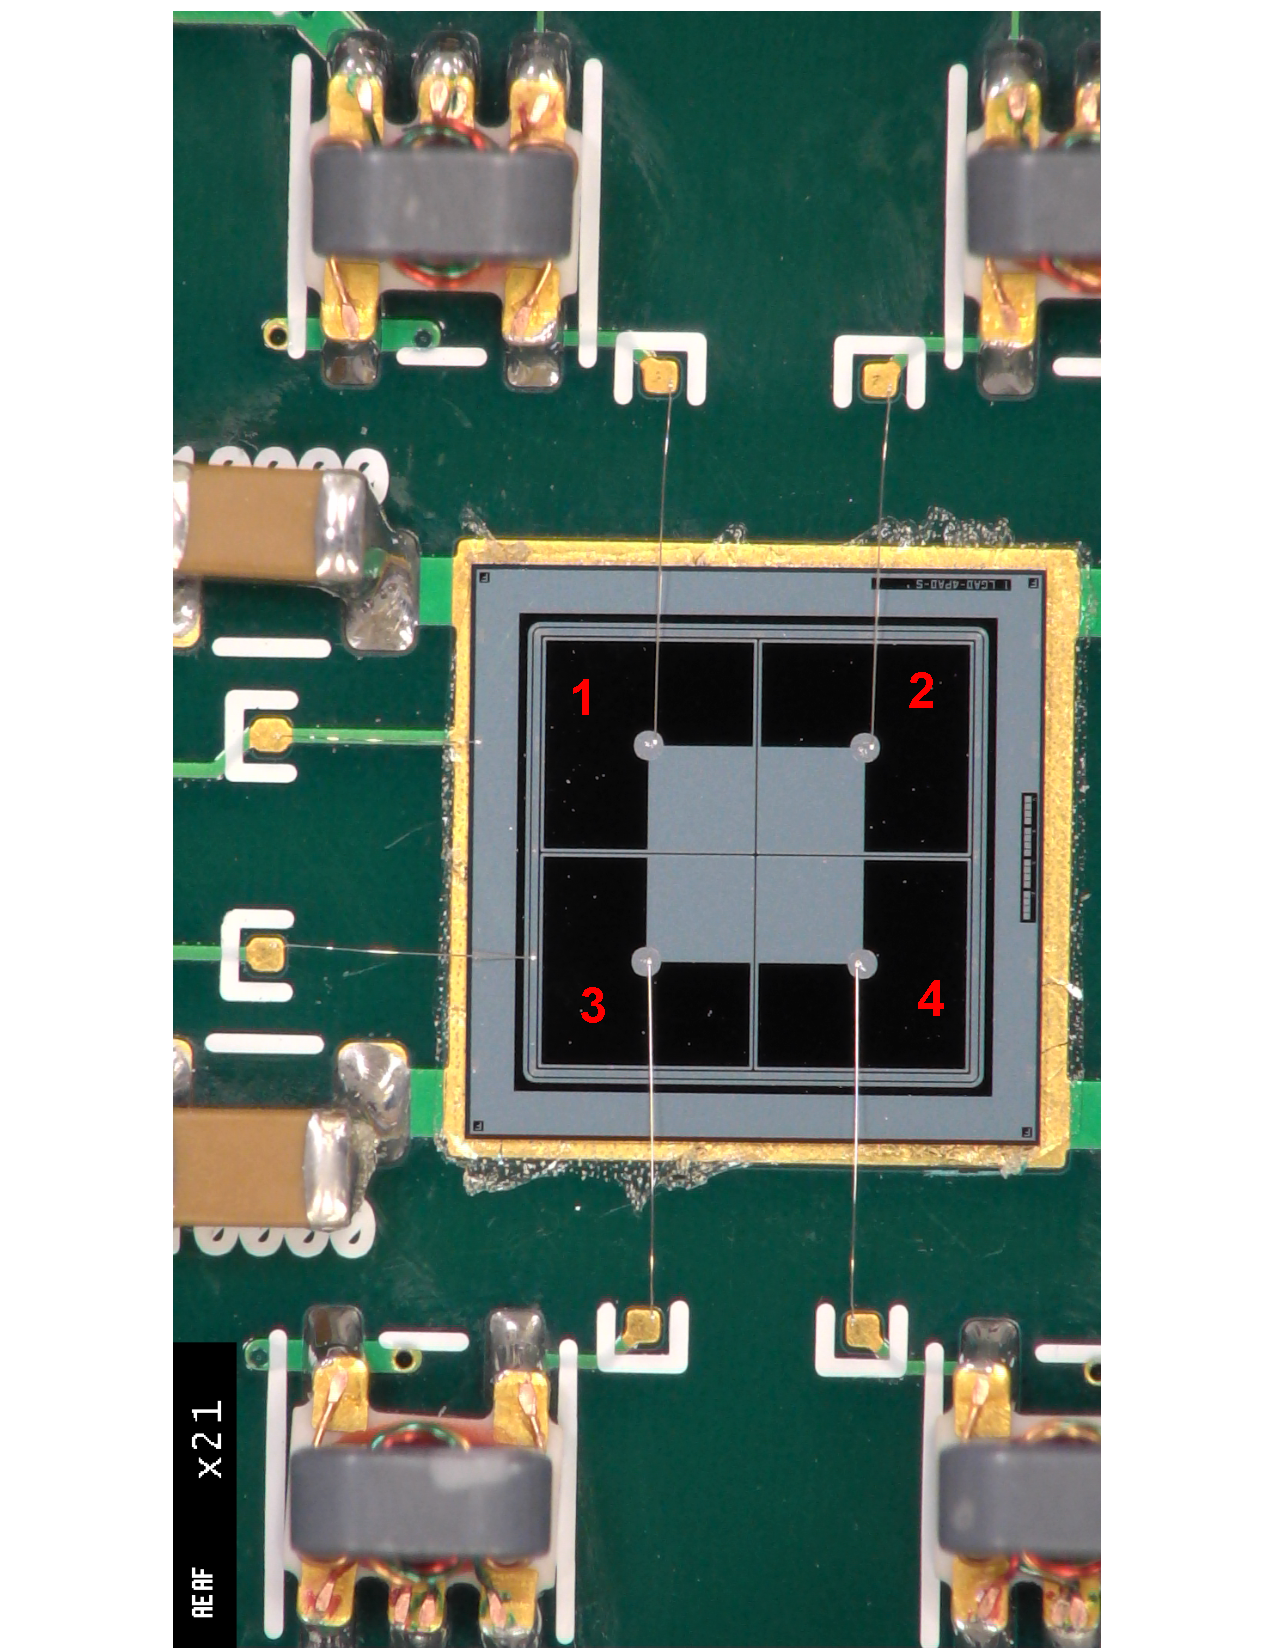
\includegraphics[width=0.41\textwidth]{figs/HPK-50D.pdf} 
\caption{A picture of HPK 50D-PIX 2x2 array sensor (top), and 50D-GR single sensor (bottom). The pixel labels overlaid on top of the left image are used in the text to identify pixels on the array. Signals from the pixels are read out by the micro-bonds that are connected to the signal pads on the sensors. Signal pads can be seen on the left photograph as four small circles in the center of each pixel. } 
\label{fig:HPK_Sensors} 
\end{figure} 





\section{Read-out boards}
\label{sec:boards}

Three boards were used in various measurements presented in this paper, which
were developed at the University of California Santa Cruz (UCSC), University of
Kansas (KU), and at FNAL:

\textbf {FIXME SERGEY} a paragraph describing the FNAL board. 

The 2-channel KU board, designed and produced by the University of Kansas, can
accommodate different types of sensors, i.e. diamond, silicon, LGAD or APDs. The
sensor is hosted on the board itself and the electronics of the version used for
this work was optimized for precise timing measurements. In particular, the
amplifier, made with discrete components, has an input impedance of 700 Ohm, an
output noise of 4 mV and a gain in transresistance of about 50 mV/$\mu$A with
a 3 dB bandwidth of 100 MHz. Those values were simulated for an input
capacitance of 20 pF, which corresponds roughly to a UFSD of 9 mm$^2$. The power
consumption of the board is about 130 mW per channel. Similar electronics is
available in different configurations with 1, 2 (used in this work) or 8
channels.

The USCS board 1-channel board is described in details in
Ref.~\cite{Cartiglia201783}. This board uses discrete components and contains
several features which allow maintaining a wide bandwidth ($\sim$ 2 GHz) and a
low noise even in noisy environments. The inverting amplifier uses a high-speed
SiGe transistor which has a trans-impedance of about 470~$\Omega$. A commercial
inverting amplifier with gain 10x is used to boost the signal. The 4-channel
UCSC board has two stages: the first one is identical to the UCSC single channel
board, and is followed by an inverting stage. The total trans-impedance is 10.7
k$\Omega$.

%\textbf {FIXME HARTMUT} a paragraph describing the 4-ch UCSC board. 


\section{Beam test results}
\label{sec:results}

\subsection{Analysis procedure}

The CAEN digitizer is voltage and time calibrated using the procedure described
in Ref.~\cite{Kim201467}. The time for the reference Photek MCP-PMT detector is
obtained by fitting the peak region of the pulse to a Gaussian function and the
mean parameter of the Gaussian is assigned as the timestamp $t_0$. The time for
signals from the LGAD sensors is obtained by performing a linear fit to the
rising edge of the pulse and the time at which the pulse reaches 30\% of the
maximum amplitude is assigned as its timestamp $t1$ \textbf{FIXME DESCRIBE THE
ALGORITHMS FOR LGADS}. We measured the electronic time resolution of the CAEN
V1742 digitizer as $\sim$4~ps and neglected its impact on the timing
measurements described below. 

Events are required to have a signal in the Photek MCP-PMT consistent with a MIP
signal, and a signal above the noise in LGAD sensors. The MIP signal selection
in Photek MCP-PMT is the same for all runs, since it was always read out
directly by the CAEN digitizer. The signal selection for LGAD boards was
optimized for each board individually, by selecting the MIP signal peak fitted
with a Landau function. 


\subsection{Study of the uniformity of the LGAD sensors}

The uniformity of the HPK 50D-PIX sensors was studied using the FNAL readout
board. Here, and in the remainder of this article, whenever a scan of a certain
characteristic quantity (e.g. time resolution) sensors is presented, we show the
X-axis scan for pixels 1 and 2, and the Y-axis scan for pixels 1 and 3, as
defined on the left picture in Fig.~\ref{fig:HPK_Sensors}. The X-axis scan
across pixels 3 and 4, and Y-axis scans across pixels 2 and 4 shown
qualitatively the same features, and are not shown here. 

The measurements of the particle detection efficiency are shown in
Fig.~\ref{fig:FNAL_HPK50_effXY}. Efficiency is defined as the ratio of events
that register a signal above the noise level in the LGAD sensor to those that
contain a track identified by the pixel telescope pointing at the LGAD sensor.
We observe a flat 100\% efficiency across the whole sensor area. The left edge
of the pixel 1 in Fig.~\ref{fig:FNAL_HPK50_effXY} is outside the acceptance of
the pixel telescope, hence the efficiency curve does not fully cover its
surface. A clear drop in efficiency is observed in the transition region between
the two pixels. The area between two pixels is shown in more detail in
Fig.~\ref{fig:FNAL_HPK50_ZoomeffXY}. In order to estimate the area with no
response between the pixels, the efficiency curves of the two neighboring pixels
are fitted with an S-curve function of the form $y=p_1\times
\mathrm{erf}\left\{\pm(p_2-x)/p_3)\}+p_4$, where $\mathrm{erf}}$ is the error
function, and $p_i$ are floated in the fit. We define as the width of the
``no-response'' area the distance between the half-maxima of the two fitted
S-curves, as shown in Fig.~\ref{fig:FNAL_HPK50_ZoomeffXY}

\begin{figure}[htbp] 
\centering
\includegraphics[width=0.48\textwidth]{figs/FNALBoard_HPK50DPix_Run847-891/Eff_vs_X_Ch4_5.pdf} 
\includegraphics[width=0.48\textwidth]{figs/FNALBoard_HPK50DPix_Run847-891/Eff_vs_Y_Ch3_4.pdf} 
\caption{Efficiency measurement across the X- and Y-axes of the HPK 50D-PIX sensor mounted on the FNAL board. The scan of pixels 1 and 2 along the X-axis, and pixels 1 and 3 along the Y-axis is shown, and pixel numbering scheme is defined in Fig.~\ref{fig:HPK_Sensors}.} 
\label{fig:FNAL_HPK50_effXY} 
\end{figure} 

\begin{figure}[htbp] 
\centering
\includegraphics[width=0.48\textwidth]{figs/KUBoard_HPK50DPix_Run638-781/EfficiencyInGap_HPK50DPix_fit.pdf} 
\caption{A zoomed version of the efficiency measurement across the X-axis of the HPK 50D-PIX sensor operated at -300 V bias voltage. Pixel numbering scheme is defined in Fig.~\ref{fig:HPK_Sensors}.} 
\label{fig:FNAL_HPK50_ZoomeffXY} 
\end{figure} 

\begin{figure}[htbp] 
\centering
\includegraphics[width=0.48\textwidth]{figs/UCSCBoard_HPK50CPix_CNM_W9HG11_Runs838-839-841/Eff_vs_X_Ch1_4_fit.pdf} 
\includegraphics[width=0.48\textwidth]{figs/UCSCBoard_HPK50CPix_CNM_W9HG11_Runs838-839-841/Eff_vs_Y_Ch3_4_fit.pdf} 
\includegraphics[width=0.48\textwidth]{figs/UCSCBoard_HPK50CPix_CNM_W9HG11_Runs838-839-841/Eff_vs_X_Ch10-13_fit.pdf} 
\includegraphics[width=0.48\textwidth]{figs/UCSCBoard_HPK50CPix_CNM_W9HG11_Runs838-839-841/Eff_vs_Y_Ch12-13_fit.pdf} 

\caption{A zoomed version of the efficiency measurement across the X- and Y-axes of the HPK 50D-PIX (top) and CNM W9HG11 (bottom) sensors. HPK sensor is operated at -450 V, and CNM sensor is at -180 V bias voltage. Data points in blue are those from one pixel, and red points are those from the neighboring pixel. The red curves are fitted to the data points as described in the text. Arrows indicate the distance between half-maximum points of fitted curves.} 
\label{fig:UCSC_HPK50C_CNM_ZoomeffXY} 
\end{figure} 


An important characteristic of the sensors is the uniformity of the signal size
across the sensor surface, which directly impacts the timing characteristics of
the sensor. The distribution of the LGAD signal amplitudes is fit with a Landau
distribution. The post-fit Most Probable Value (MPV) is
plotted in Fig.~\ref{fig:FNAL_HPK50_MPVXY}. A flat response with a uniform
signal size is observed over the whole sensor area.

\begin{figure}[htbp] 
\centering
\includegraphics[width=0.48\textwidth]{figs/FNALBoard_HPK50DPix_Run847-891/MPV_vs_X_Ch4_5.pdf} 
\includegraphics[width=0.48\textwidth]{figs/FNALBoard_HPK50DPix_Run847-891/MPV_vs_Y_Ch3_4.pdf} 
\caption{Signal amplitude MPV measurement across the X- and Y-axes of the HPK 50D-PIX sensor mounted on the FNAL board. The scan of pixels 1 and 2 along the X-axis, and pixels 1 and 3 along the Y-axis is shown, and pixel numberng scheme is defined in Fig.~\ref{fig:HPK_Sensors}.} 
\label{fig:FNAL_HPK50_MPVXY} 
\end{figure} 



The measurement of the time difference between the Photek 240 MCP-PMT time
stamp, and that of the LGAD sensors is shown in Fig.~\ref{fig:FNAL_HPK50_DTXY}.
The micro-bonding scheme of the HPK PIX $2\times 2$ sensors arrays is shown in
Fig.~\ref{fig:HPK_Sensors}. The $\Delta t = t_{1}-t_{0}$ distribution has a
distinct shape where the area under the metallization on top of the sensor -- the
gray area in the center of the image -- shows a shift of about $20$--$30$~ps with
respect to non-metallized area. A possible explanation for this small effect is
an observed slight difference in the rise time of pulse from the metallized and
un-metallized areas. 

\begin{figure}[htbp] 
\centering
\includegraphics[width=0.48\textwidth]{figs/FNALBoard_HPK50DPix_Run847-891/MeanTime_vs_X_Ch4_5.pdf} 
\includegraphics[width=0.48\textwidth]{figs/FNALBoard_HPK50DPix_Run847-891/MeanTime_vs_Y_Ch3_4.pdf} 
\caption{$\Delta t$ measurement across the X- and Y-axes of the HPK 50D-PIX sensor mounted on the FNAL board. The scan of pixels 1 and 2 along the X-axis, and pixels 1 and 3 along the Y-axis is shown, and pixel numberng scheme is defined in Fig.~\ref{fig:HPK_Sensors}.} 
\label{fig:FNAL_HPK50_DTXY} 
\end{figure} 

The measurement of the time resolution scan across the sensor is shown in
Fig.~\ref{fig:FNAL_HPK50_SigmaTXY}. The $\Delta t$ distribution between LGAD
sensor and the Photek 240 MCP-PMT sensor is fitted with a Gaus function, and its
spread $\sigma$ is referred to in the following as the time resolution. We
observe a uniform time resolution around 40~ps across the whole sensor area. 

\begin{figure}[htbp] 
\centering
\includegraphics[width=0.48\textwidth]{figs/FNALBoard_HPK50DPix_Run847-891/TimeResolution_vs_X_Ch4_5.pdf} 
\includegraphics[width=0.48\textwidth]{figs/FNALBoard_HPK50DPix_Run847-891/TimeResolution_vs_Y_Ch3_4.pdf} 
\caption{Time resolution measurement across the X- and Y-axes of the HPK 50D-PIX sensor mounted on the FNAL board. The scan of pixels 1 and 2 along the X-axis, and pixels 1 and 3 along the Y-axis is shown, and pixel numberng scheme is defined in Fig.~\ref{fig:HPK_Sensors}.} 
\label{fig:FNAL_HPK50_SigmaTXY} 
\end{figure} 


%\subsection{Comparison of the boards}


\subsection{Comparison of HPK doping profiles}

Studies of the dependence of the timing sensors characteristics on the sensor
doping were performed by comparing the 50~$\mu$m PIX sensors of different gain
splits. All measurements were performed using 2-channel KU readout board. 

\begin{figure}[htbp] 
\centering
\includegraphics[width=0.9\textwidth]{figs/KUBoard_HPK50ABCD/KUBoard_50ABCD_TimeResolution.pdf} 
\caption{Time resolution on KU board with 50A, B, C, D } 
\label{fig:Sensors} 
\end{figure} 

\begin{figure}[htbp] 
\centering
\includegraphics[width=0.9\textwidth]{figs/KUBoard_HPK50ABCD/KUBoard_50ABCD_MeanTime.pdf} 
\caption{DeltaT on KU board with 50A, B, C, D } 
\label{fig:Sensors} 
\end{figure} 

\begin{figure}[htbp] 
\centering
\includegraphics[width=0.9\textwidth]{figs/KUBoard_HPK50ABCD/KUBoard_50ABCD_MPV.pdf} 
\caption{MPV on KU board with 50A, B, C, D } 
\label{fig:Sensors} 
\end{figure} 



\subsection{Comparison of HPK 50 $\mu$m with 80 $\mu$m}
\label{sec:HPK50vs80}

\begin{figure}[htbp] 
\centering
\includegraphics[width=0.7\textwidth]{figs/FNAL_TimeResolution_vs_X_HPK50CVs80C.pdf} 
\caption{Comparison of time resolution in FNAL 80C versus KU 50C sensors } 
\label{fig:Sensors} 
\end{figure} 


\subsection{Temperature dependence of the LGAD sensors}

\begin{figure}[htbp] 
\centering
\includegraphics[width=0.9\textwidth]{figs/FNAL_TimeResolution_vs_X_HPK50D_TemperatureDependance.pdf} 
\caption{Time resolution on FNAL board with 50D at +20, -10, -20C} 
\label{fig:Sensors} 
\end{figure} 

\begin{figure}[htbp] 
\centering
\includegraphics[width=0.9\textwidth]{figs/FNAL_MeanTime_vs_X_HPK50D_TemperatureDependance.pdf} 
\caption{DeltaT on FNAL board with 50D at +20, -10, -20C} 
\label{fig:Sensors} 
\end{figure} 


\begin{figure}[htbp] 
\centering
\includegraphics[width=0.9\textwidth]{figs/FNAL_MPV_vs_X_HPK50D_TemperatureDependance.pdf} 
\caption{MPV on FNAL board with 50D at +20, -10, -20C} 
\label{fig:Sensors} 
\end{figure} 

\subsection{Radiation tolerance of the LGADs up to 6$\times 10^{14}$}

\begin{figure}[htbp] 
\centering
\includegraphics[width=0.48\textwidth]{figs/USCSBoard_HPK50DIrradiated-CNMW11LGA35_Run936-961/CNM_irradiated_amp_Map.pdf} \hfill
\includegraphics[width=0.48\textwidth]{figs/USCSBoard_HPK50DIrradiated-CNMW11LGA35_Run936-961/CNM_irradiated_amp_1D.pdf} 
\caption{(Left) The map of the amplitude distribution on the irradiated CNM W11LGA35 sensor across X and Y coordinates. Two distinct regions on the sensor surface can be identified according to the amplitude distribution: the center of the sensor (area within the red circle), and the periphery of the sensor (area between the black circle and black square). (Right) Amplitude distribution in the two areas of the irradiated CNM W11LGA35 sensor.} 
\label{fig:Sensors} 
\end{figure} 

\begin{figure}[htbp] 
\centering
\includegraphics[width=0.48\textwidth]{figs/USCSBoard_HPK50DIrradiated-CNMW11LGA35_Run936-961/HPK_irradiated_amp_Map.pdf} \hfill
\includegraphics[width=0.48\textwidth]{figs/USCSBoard_HPK50DIrradiated-CNMW11LGA35_Run936-961/HPK_irradiated_amp_1D.pdf} 
\caption{(Left) The map of the amplitude distribution on the irradiated HPK 50D sensor across X and Y coordinates. Two distinct regions on the sensor surface can be identified according to the amplitude distribution: the center of the sensor (area within the red circle), and the periphery of the sensor (area between the black circle and black square). (Right) Amplitude distribution in the two areas of the irradiated HPK 50D sensor.} 
\label{fig:Sensors} 
\end{figure} 

\begin{figure}[htbp] 
\centering
\includegraphics[width=0.90\textwidth]{figs/USCSBoard_HPK50DIrradiated-CNMW11LGA35_Run936-961/IrradiatedSensorStudy_Efficiency_vs_X.pdf} 
\includegraphics[width=0.90\textwidth]{figs/USCSBoard_HPK50DIrradiated-CNMW11LGA35_Run936-961/IrradiatedSensorStudy_Efficiency_vs_Y.pdf} 
\caption{Efficiency vs X and Y on CNM and HPK irradiated} 
\label{fig:Sensors} 
\end{figure} 

\begin{figure}[htbp] 
\centering
\includegraphics[width=0.90\textwidth]{figs/USCSBoard_HPK50DIrradiated-CNMW11LGA35_Run936-961/IrradiatedSensorStudy_MPV_vs_X.pdf} 
\includegraphics[width=0.90\textwidth]{figs/USCSBoard_HPK50DIrradiated-CNMW11LGA35_Run936-961/IrradiatedSensorStudy_MPV_vs_Y.pdf} 
\caption{MPV vs X and Y on CNM and HPK irradiated} 
\label{fig:Sensors} 
\end{figure}


\begin{figure}[htbp] 
\centering
\includegraphics[width=0.90\textwidth]{figs/USCSBoard_HPK50DIrradiated-CNMW11LGA35_Run936-961/IrradiatedSensorStudy_TimeResolution_vs_X.pdf} 
\includegraphics[width=0.90\textwidth]{figs/USCSBoard_HPK50DIrradiated-CNMW11LGA35_Run936-961/IrradiatedSensorStudy_TimeResolution_vs_Y.pdf} 
\caption{Time Resolution vs X and Y on CNM and HPK irradiated} 
\label{fig:Sensors} 
\end{figure} 

\begin{figure}[htbp] 
\centering
\includegraphics[width=0.9\textwidth]{figs/USCSBoard_HPK50DIrradiated-CNMW11LGA35_Run936-961/IrradiatedSensorStudy_MeanTime_vs_X.pdf} 
\includegraphics[width=0.9\textwidth]{figs/USCSBoard_HPK50DIrradiated-CNMW11LGA35_Run936-961/IrradiatedSensorStudy_MeanTime_vs_Y.pdf} 
\caption{DeltaT vs X and Y on CNM and HPK irradiated} 
\label{fig:Sensors} 
\end{figure} 
 

\section{Conclusion}
\label{sec:conclusion} 

In a beam test at FNAL with tracking information, we compared the performance of
low-gain avalanche detectors (LGAD) produced by CNM Barcelona and HPK Hamamatsu,
both single pads and 2x2 arrays with pad size varying from 1 mm to 3 mm diameter
and a thickness of about 50 and 80 $\mu$m. Four different readout boards were
used, and their performance characteristics will be detailed in an upcoming
paper. The uniformity of the sensor response in pulse height, efficiency and
timing resolution were tested and found to be good pre-radiation with the
exceptions of the area between pads which exhibit a ``no-response'' width of
72.5~$\mu$m for CNM and 112.7~$\mu$m for HPK. A small timing shift across the
HPK sensor of the order 20--30~ps can be explained by the observed change in
pulse shape when comparing metallized and non-metallized sensor areas. After a
neutron fluence of $6\times 10^{14}$~n/cm$^2$, the single pad CNM sensor
exhibits a large gain variation of a factor 2.5 when comparing metallized and
non-metallized sensor areas. 

For an un-irradiated 50~$\mu$m thick LGAD with 3~mm pads we find the following timing results: 
\begin{itemize}
  \item at a temperature of $+20$~C$^{\circ}$, the timing resolution ranges from
        40~ps to 50~ps depending on the readout board. This number worsens by
        10~ps for a 80~$\mu$m sensor.
  \item cooling the LGAD improves the timing resolution from 55~ps at
        $+20$~C$^{\circ}$ to 43~ps at $-10$~C$^{\circ}$ to 36 ps at
        $-20$~C$^{\circ}$  
\end{itemize}

For an 50~$\mu$m thick LGAD with 1~mm pads irradiated $6\times 10^{14}$~n/cm$^2$ we find the
following timing results when operated at $-20$~C$^{\circ}$: 
\begin{itemize}
  \item for the HPK LGAD the highest bias voltage reached is $\sim$600V and the timing resolution is 30~ps; 
  \item for the CNM LGAD the highest bias voltage reached is $\sim$400V and the
        timing resolution is 30~ps for the metallized part and~40 ps for the
        un-metallized area.
  
\end{itemize}






\section*{Acknowledgement}

We would like to thank Alan Prosser and Ryan Rivera for their critical help in
setting up the DAQ and trigger chain. 

We thank Ned Spencer, Max Wilder, and Forest McKinney-Martinez for their
technical assistance, and the CNM and HPK manufacturing team. We acknowledge the
help of V. Cindro and I. Mandic with the neutron irradiations. Part of this work
has been performed within the framework of the CERN RD50 Collaboration. The work
was supported by the United States Department of Energy, grant
DE-FG02-04ER41286. Part of this work has been financed by the European Union’s
Horizon 2020 Research and Innovation funding program, under Grant Agreement no.
654168 (AIDA-2020) and Grant Agreement no. 669529 (ERC UFSD669529), and by the
Italian Ministero degli Affari Esteri and INFN Gruppo V.



%% The Appendices part is started with the command \appendix;
%% appendix sections are then done as normal sections

\appendix
\section{Appendix A}

The list of sensors studied in this article, as well as the temperature and the
sensor bias voltage used during their operation are listed in
Tab.~\ref{tab:DataConditions}. 

\begin{table}[h]
\begin{center}
  \begin{tabular}{ |c | c | c| c | }
    \hline
    Sensor      & KU Board 2-ch & UCSC board 4-ch & FNAL board 4-ch \\ \hline \hline
    HPK 50A-PIX & {\textbf{-630 V} & -- & -- \\ \hline
    HPK 50B-PIX & \begin{tabular}{@{}c@{}}{\textbf{-450 V, -550V, -600 V }\\ \underline{-510 V} \\ \textit{-510V, -570 V}\end{tabular}  & -- & -- \\ \hline
    HPK 50C-PIX & {\textbf{-400 V} & {\textbf{-410 V, -470 V} & -- \\ \hline
    HPK 50D-PIX & \begin{tabular}{@{}c@{}}{\textbf{-100 V, -200V, -250 V,} \\ \textbf{-300 V, -325 V} \end{tabular}  & -- & \begin{tabular}{@{}c@{}}{\textbf{-250 V, -300V,} \\ \underline{-210 V, -250 V} \\ \textit{-250 V, -280 V}\end{tabular} {\color{red}} \\ \hline
    CNM W9HG11 & -- & {\textbf{-140 V, -160V} & -- \\ \hline
    \begin{tabular}{@{}c@{}}HPK 50D \\  $6\times 10^{14}$~n/cm$^2$ \end{tabular} & -- & {\textit{-600 V, -635V} & -- \\ \hline
    \begin{tabular}{@{}c@{}}CNM W11LGA35 \\ $6\times 10^{14}$~n/cm$^2$ \end{tabular} & -- & -- & {\textit{-400 V, -420V} \\ \hline
    \hline
  \end{tabular}
\caption{Data taking conditions for the studies presented in this paper. Numbers in bold indicate that the sensor was at  room temperature, underlined ones were taken at $-10$C$^{\circ}$, and those in italicized text were taken at $-20$C$^{\circ}$.}  
\label{tab:DataConditions}
\end{center}
\end{table}

%% \section{}
%% \label{}

%% If you have bibdatabase file and want bibtex to generate the
%% bibitems, please use
%%
%%  \bibliographystyle{elsarticle-num} 
%%  \bibliography{<your bibdatabase>}

%% else use the following coding to input the bibitems directly in the
%% TeX file.

\bibliography{LGAD_May2017_FNALTB}{}
\bibliographystyle{ieeetr} 

%\begin{thebibliography}{00}

%% \bibitem{label}
%% Text of bibliographic item

%\bibitem{}

%\end{thebibliography}
\end{document}
\endinput
%%
%% End of file `elsarticle-template-num.tex'.


























